
%%%%%%%%%%%%%%%%%%%%%%%%%%%%%%%%%%%%%%%%%%%%%%%%%%%%%%%%%%%%%%%%%%%%%%%%%%%%%%%%%%%%%%%%%%%%%%%%%%%%%%%%%%%%%%%


\begin{figure}[h!]

\begin{center}

    \caption{Calculation of Kullback-Leibler Distance} \label{fig:KLDdistance1}

        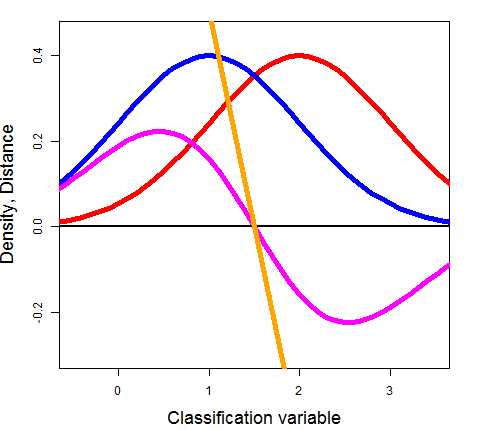
\includegraphics[scale=  0.50]{Figs/KLD/KLD_calc_3.png}



\end{center}

    \footnotesize

        \textbf{Terms in the Calculation of Kullback-Leibler Distance:}
        Differences (magenta) and log-differences (orange) for two normal densities (red and blue). 
        Notice that the difference is damped where density is low, while the log-difference grows linearly. 
        This places greater emphasis on areas of support with low density. 

% Terms in $KLD(\textcolor{blue}{f_1}, \textcolor{red}{f_2})
%  = \sum_{k = 1}^{K} \left\{ \textcolor{magenta}{\big( f_1(t_k) - f_2(t_k) \big)}
%         \textcolor{orange}{\log \left( \frac{f_1(t_k)}{f_2(t_k)} \right)} \right\}$

\end{figure}


%%%%%%%%%%%%%%%%%%%%%%%%%%%%%%%%%%%%%%%%%%%%%%%%%%%%%%%%%%%%%%%%%%%%%%%%%%%%%%%%%%%%%%%%%%%%%%%%%%%%%%%%%%%%%%%

